\documentclass{beamer}
\usetheme{Boadilla}
\usepackage{graphicx}
\usepackage{amsmath}
\usepackage{mathtools}
\usepackage{xmpmulti}
\usepackage[T1]{fontenc}
\usepackage[ansinew]{inputenc}

%path and template
\graphicspath{{./images/}}
\setbeamertemplate{caption}[numbered]

%info
\title{Air Quality Monitoring Wireless System}
\author{Graziano A. Manduzio, PhD student}
\institute{University of Florence}
\date{\today}

%newcommand
\newcommand{\B}{\pmb{B}}
\newcommand{\mb}{\mathbf}
\newcommand{\bs}{\boldsymbol}

\begin{document}
%%%%%%%%%%%%%%%%%%%%%%%%%%%%%%%%%%%%%%%%%%%%%%%%%%%%%%%%%%%%%%%%%%%%%
\begin{frame}
	\titlepage
	\center{supervisors: Giorgio Battistelli, Luigi Chisci ,Nicola Forti and Roberto Sabatini}
\end{frame}
%%%%%%%%%%%%%%%%%%%%%%%%%%%%%%%%%%%%%%%%%%%%%%%%%%%%%%%%%%%%%%%%%%%%%
\begin{frame}{Model}
Advection-diffusion model equation: second order pde equation
\begin{equation}
		\displaystyle{\frac{\partial x}{\partial t}} - \lambda \nabla^2 x + \mb{v}^T \nabla x  ~=~ f \,\,\,\,\, \mbox{in } \mathbb{R}^2
\end{equation}
where:\\
	$x(\mb{p},t)$ is the space-time dependent pollutant concentration field, defined over the space-time domain with an initial condition $x(\mb{p},0)=x_{0}$;\\
	$\mb{p} \in \mathbb{R}^2$ denotes the $2$-dimensional position vector;\\
	$t \in \mathbb{R}^{+}$ denotes time;\\
	$\lambda$ is the diffusion coefficient;\\
	$\mb{v}(\mb{p},t)$ is the advection velocity vector;\\
	$f(\mb{p},t)=s(t)F(\mb{p})$ represents the internal sources of pollution, defined as the product of the source signal waveform $s(t)$ and the position-dependent function $F(\mb{p})$.\\
	We need to truncate the physical domain to solve numerically the problem by using the finite element method (FEM): $\mathbb{R}^2 -> \Omega$.
\end{frame}
%%%%%%%%%%%%%%%%%%%%%%%%%%%%%%%%%%%%%%%%%%%%%%%%%%%%%%%%%%%%%%%%%%%%%%
\begin{frame}{Variational formulation of the problem}
\[
	\int_\Omega \frac{\partial x}{\partial t} \varphi \, d\mb{p} \, - \,
	\lambda \int_\Omega ~\nabla^2 x~ \varphi \, d\mb{p} +
	\int_\Omega \mb{v}^T  ~\nabla x~ \varphi \, d\mb{p} =
	\int_\Omega f \varphi \, d\mb{p}
	\]
	where $\varphi(\mb{p})$ is a generic space-dependent weight function.
\\ 	
\vspace{2mm}
Green's identity substitution\\
$\varphi \nabla^2 x = \nabla . (\varphi \nabla x) - \nabla \varphi . \nabla x$\\

\[
\begin{array}{l}
	\displaystyle
	\int_\Omega \frac{\partial x}{\partial t} \varphi \, d\mb{p} \, - \,
	\lambda \int_\Omega \nabla . (\varphi \nabla x) \, d\mb{p} + \lambda \int_\Omega \nabla \varphi . \nabla x \, d\mb{p} +
	\int_\Omega \mb{v}^T  ~\nabla x~ \varphi \, d\mb{p} = \\ [4mm]
	\displaystyle
	\int_\Omega f \varphi \, d\mb{p}
\end{array}
	\]\\
	
	\[
	\begin{array}{l}
	\displaystyle
	\int_\Omega \frac{\partial x}{\partial t} \varphi \, d\mb{p} \, - \,
	\lambda \int_{\partial \Omega} \varphi \nabla x . \mb{n} \, d\mb{p} + \lambda \int_\Omega \nabla \varphi . \nabla x \, d\mb{p} +
	\int_\Omega \mb{v}^T  ~\nabla x~ \varphi \, d\mb{p} = \\ [4mm]
	\displaystyle
	s(t) \int_\Omega F(\mb{p}) \varphi \, d\mb{p}
	
	\end{array}
	\]
\end{frame}

%%%%%%%%%%%%%%%%%%%%%%%%%%%%%%%%%%%%%%%%%%%%%%%%%%%%%%
\begin{frame}{FEM derivation}

FEM approximation:\\
\begin{center}

$	x(\mb{p},t) \simeq \sum_{j=1}^{n} \phi_{j}(\mb{p}) \, x_j(t) ~=~ \boldsymbol{\phi}^T(\mb{p}) \, \mb{x}(t)$

\end{center}
\vspace{0.1cm}

FEM derivative model:
a set of $n$ inhomogeneus differential equations

\begin{multline} 
\small{\underbrace{\left[ \int_\Omega  
			\bs{\phi}(\mb{p}) \,\bs{\phi}^T(\mb{p}) d\mb{p} 
			\right]}_{\mb{M}} \dot{\mb{x}}(t)  + 
		\underbrace{\left[ \lambda \int_\Omega 
			\nabla	\bs{\phi}^T(\mb{p}) \,\nabla \bs{\phi}(\mb{p}) d\mb{p} 
			\right]}_{\mb{S}_\lambda} \mb{x}(t) }\\
\small{+ \underbrace{\left[ \int_\Omega 
			\bs{\phi}(\mb{p}) ~ (\mb{v}^T(\mb{p}) \,\nabla \bs{\phi}(\mb{p}) )\, d\mb{p} 
			\right]}_{\mb{S}_\mb{v}} \mb{x}(t) }
	\small{- \underbrace{\left[ \lambda \int_{\partial \Omega} 
			 \bs{\phi}(\mb{p}) (\mb{n}^T \nabla \bs{\phi}(\mb{p})) \, d\mb{p}
			\right]}_{\mb{Q}_\lambda} \mb{x}(t) = }\\
	=  \small{\underbrace{\left[\displaystyle{\int_\Omega} \bs{\phi}(\mb{p})
			F(\mb{p}) d\mb{p}	\right]}_{\mb{f}} {s}(t) }
\end{multline} 
\end{frame}
%%%%%%%%%%%%%%%%%%%%%%%%%%%%%%%%%%%%%%%%%%%%%%%%%%%%%%%%%%%%%%%%%%%
\begin{frame}{Source terms}
example1: \\
single source\\
$f(\mb{p},t)=s(t)\delta(\mb{p}-\mb{p}_s)$\\
$$s(t)\int_\Omega \bs{\phi}(\mb{p})
			F(\mb{p}) d\mb{p} = s(t)\int_\Omega \bs{\phi}(\mb{p})
			\delta(\mb{p}-\mb{p}_s) d\mb{p}=s(t)\bs{\phi}(\mb{p}_s)$$
example2:\\
multiple point source\\
\vspace{1mm}
$f(\mb{p},t)=\sum_{s=1}^{N_s} s_s(t) \delta(\mb{p}-\mb{p}_s)$\\
$$\int_\Omega \bs{\phi}(\mb{p})
			f(\mb{p},t) d\mb{p} = \sum_{s=1}^{N_s} s_s(t) \int_\Omega \bs{\phi}(\mb{p})
			\delta(\mb{p}-\mb{p}_s) d\mb{p}= \sum_{s=1}^{N_s} s_s(t) \bs{\phi}(\mb{p}_s)$$\\
\end{frame}
%%%%%%%%%%%%%%%%%%%%%%%%%%%%%%%%%%%%%%%%%%%%%%%%%%%%%%%%%%%%%%%%%%%
\begin{frame}{Advection Diffusion Model without source}
advection velocity vector $=[5 \hspace{2mm} 5]$ m/sec.\\
diffusion coefficient $=5$ m$^2$/sec
\end{frame}
%%%%%%%%%%%%%%%%%%%%%%%%%%%%%%%%%%%%%%%%%%%%%%%%%%%%%%%%%%%%%%%%%%%
\begin{frame}{Advection Diffusion Model without source}
        \transduration<0-6>{0}
        \multiinclude[<+->][format=png, graphics={width=\textwidth}]{pics/fig}
\end{frame}
%%%%%%%%%%%%%%%%%%%%%%%%%%%%%%%%%%%%%%%%%%%%%%%%%%%%%%%%%%%%%%%%%%%
\begin{frame}{Analytical vs FEM comparison}
\center
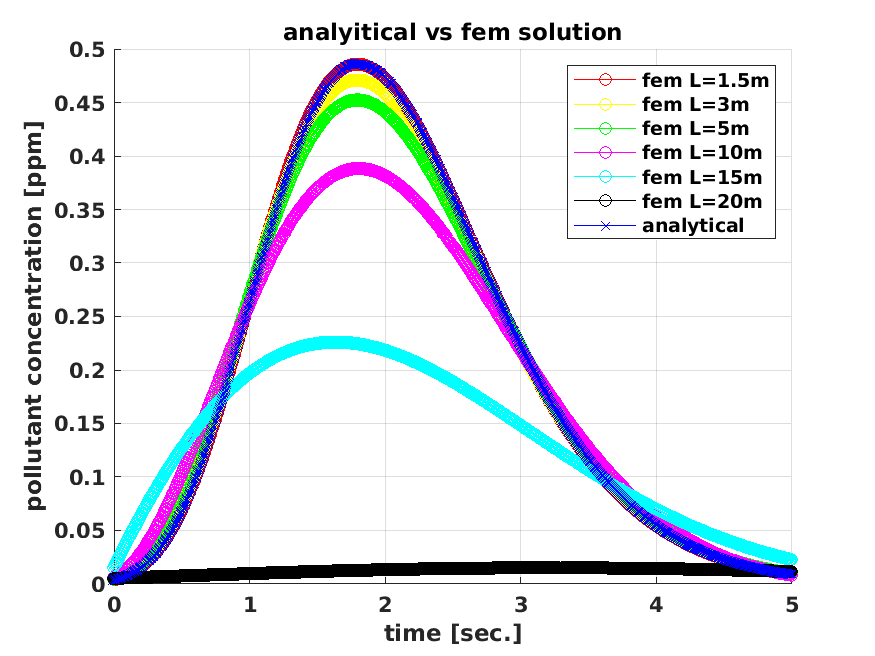
\includegraphics[scale=0.6]{pics/comparison.png}
\end{frame}
%%%%%%%%%%%%%%%%%%%%%%%%%%%%%%%%%%%%%%%%%%%%%%%%%%%%%%%%%%%%%%%%%%%
\begin{frame}{Advection Diffusion Model with sources}
advection velocity vector $=[2 \hspace{2mm} 2]$ m/sec.\\
diffusion coefficient $=0.1$ m$^2$/sec
\end{frame}
%%%%%%%%%%%%%%%%%%%%%%%%%%%%%%%%%%%%%%%%%%%%%%%%%%%%%%%%%%%%%%%%%%%%
\begin{frame}{Advection Diffusion Model with sources}
        \transduration<0-7>{0}
        \multiinclude[<+->][format=png, graphics={width=\textwidth}]{pics/sources}
\end{frame}
%%%%%%%%%%%%%%%%%%%%%%%%%%%%%%%%%%%%%%%%%%%%%%%%%%%%%%%%%%%%%%%%%%%
\begin{frame}{Domain Mesh}
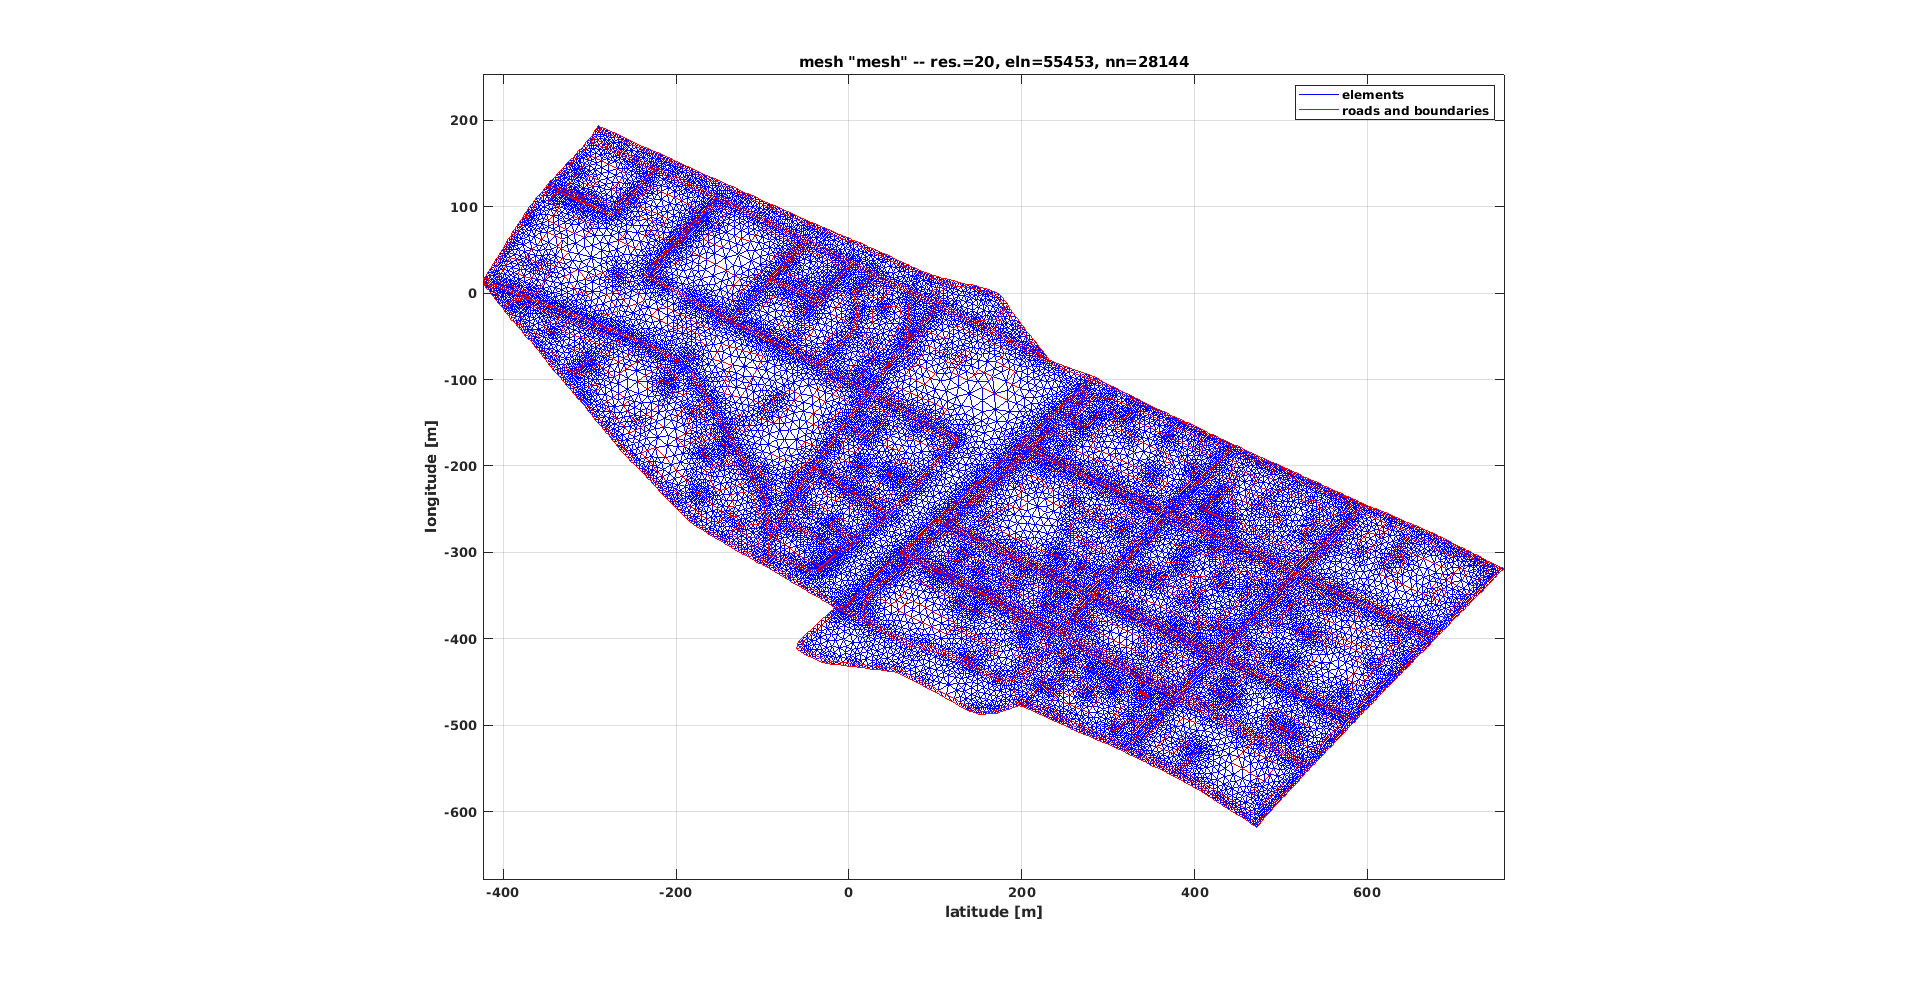
\includegraphics[width=\textwidth]{pics/mesh.png}
\end{frame}
%%%%%%%%%%%%%%%%%%%%%%%%%%%%%%%%%%%%%%%%%%%%%%%%%%%%%%%%%%%%%%%%%%%
\begin{frame}{Domain source points}
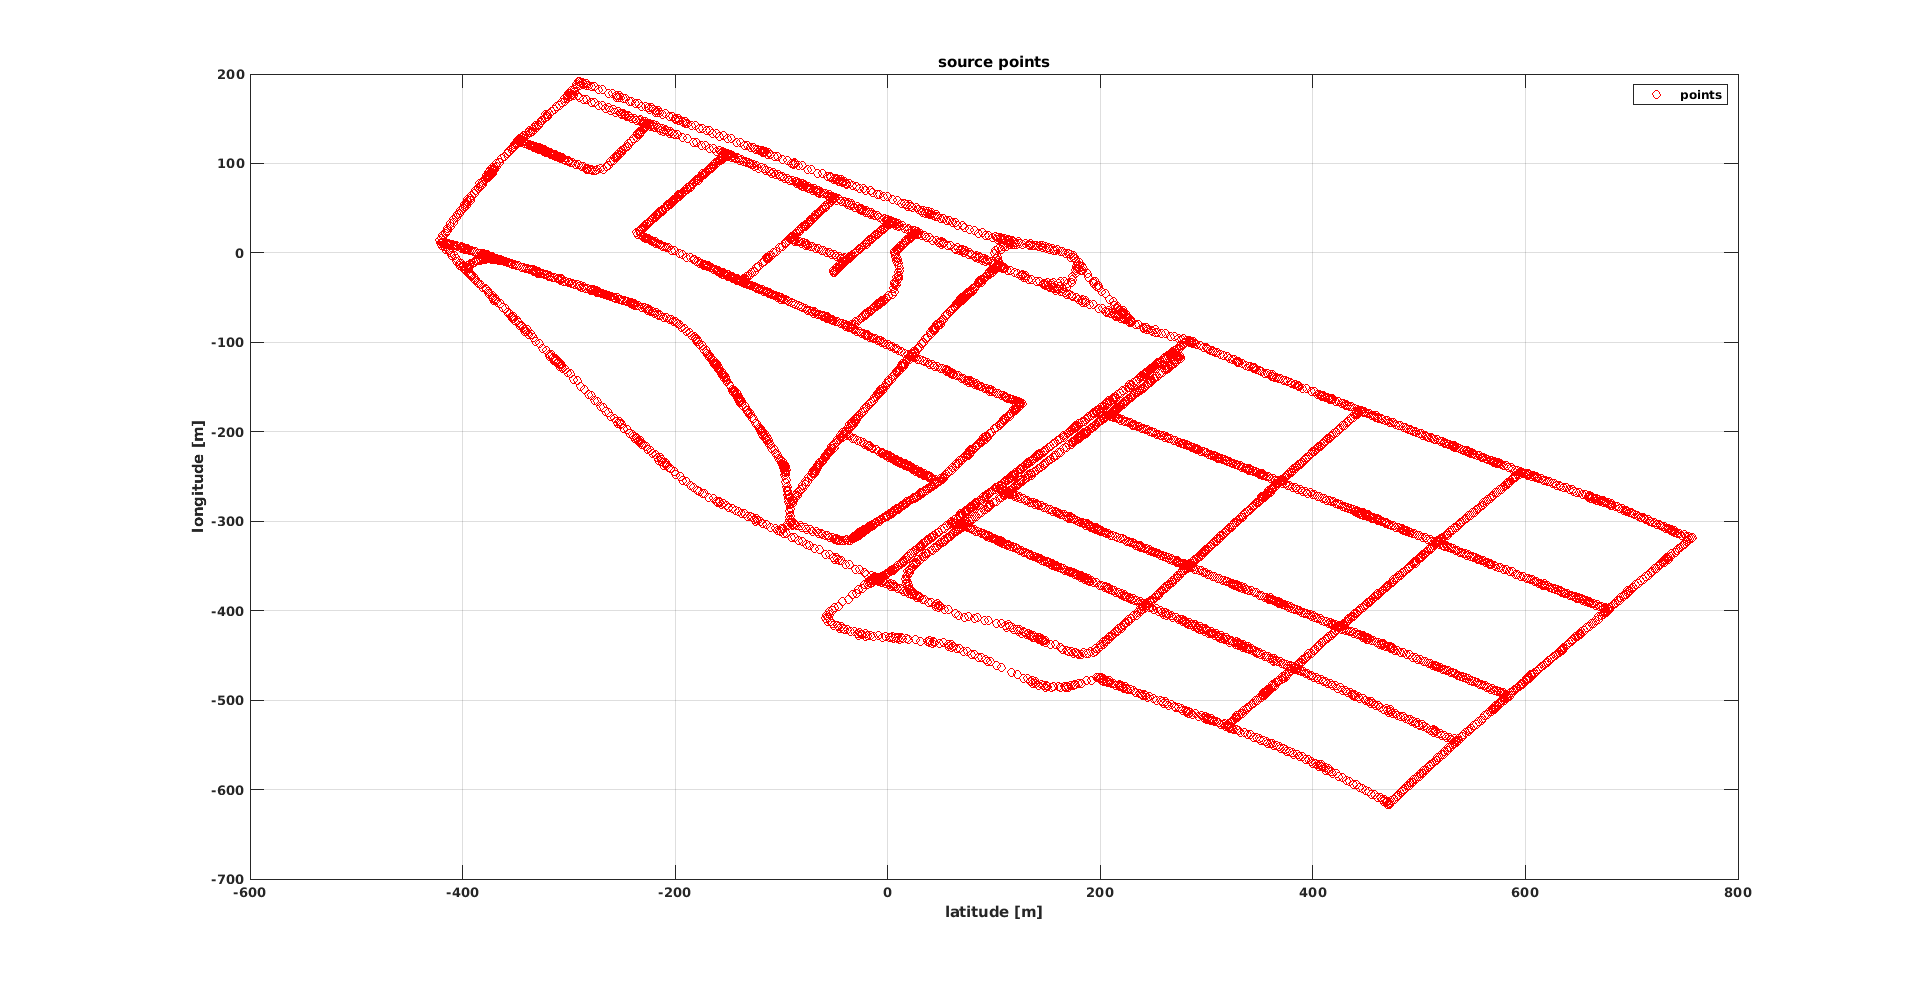
\includegraphics[width=\textwidth]{pics/source_points.png}
\end{frame}
%%%%%%%%%%%%%%%%%%%%%%%%%%%%%%%%%%%%%%%%%%%%%%%%%%%%%%%%%%%%%%%%%%%
\end{document}



	

	
